
\chapter{Background}
\label{ch:background}
\setcounter{figure}{1}      % reset the figure counter

\section{Ray Tracing Algorithm Overview}

The ray-tracing algorithm is adopted by most photorealistic rendering system to generate a highly realistic image of a 3D scene. The core concept of the ray-tracing algorithm is straightforward, it is based on shooting the ray from the view point to a 3D scene as it interacts with the objects and light source in the scene. It can be understood as the reversed process of how our eyes perceive the world, which is receiving the light rays emitted by the light source and bounced off to the eyes. To simulates the physical phenomenon, a rendering system will have to model  the following key components : 

\begin{description} 	
	\item[Camera] \hfill \\
		The camera defines the position from where the scene is being observed and how the rays are generated. As an abstraction of the real camera, the camera in the rendering sytem is typically modeled with an eye position and the image or film in front of the eye, expecting the answer to what the color to display at each point in the image? Give the eye position as the origin and a point on the image, a ray can be generated by the camera and will be shot to the scene and the ray-object intersection test can be performed to determine the color value of that point on the image.  

	\item[Scene Description] \hfill \\ 
		The ``scene'' to be rendered is conceptually a database of ``geometric primitives'', which can be from simple geometric shapes such as polygons, spheres to complex shapes such as Bezier or NURBS patches. In fact, ray tracing can handle \emph{any} type of primitives as long as there is a proper algorithm to compute and intersection between ray and the primitive.

		Choosing the types of geometric primitive the ray tracer is going to support is an important design decision to make. The ray tracer can directly support complex primitives without tessellating them into polygon, thus they can be ray traced very efficiently and accurate, for example, directly compute the intersection between the ray and a sphere is almost trivial, while a tessellated sphere requires hundreds of triangles for a reasonable accuracy. However, the ray tracer that only supports these high-level primitives suffers from huge complexity and poor maintainability. Specific routine has to be implemented to support new type of primitive. On the other hand, supporting only triangles leads to a simple and optimized ray tracer implementation, the intersection calculation routine between a ray and triangle is quite efficient. Furthermore, triangle-based mesh can be used to approximate all of the high-level primitives very well and has a widely usage in the industrial application such as video games, CAD and movies. In conclusion, a triangle-based ray tracer is a more preferable design due to its simplicity and usability.

	\item[Ray Casting] \hfill \\
		Ray casting, the key problem for a ray-tracer to solve, is to shoot rays through each pixels on the image into the scene and then find out which geometric primitive, if any, that the ray hit first and where intersection point is. All the objects in the scene will be tested against the ray the first one will be selected. Given a ray \(r\) in parametric form:
		\begin{equation}
			r(t) = o + td
		\end{equation}
		where \( o \) is the ray's origin and \( d \) is the direction vector which is usually normalized so that the parameter \( t \) can be simply treated as the distance from the origin. The valid range of \( t \) is \( [0, \infty] \). With surface defined by an implicit function \( F(x, y, z) = 0 \), it is easy to find the intersection point by substituting the ray equation into the implicit equation to obtain a new function whose only parameter is \( t \), solving this function for \( t \), and substitute the smallest positive root into the ray equation to find the desired point. If there are no positive roots, the ray must miss the surface. The intersection point is not sufficient, ray-tracer also needs to know the additional properties of the surface such as normal vector and materials at that point to perform the shading stage later.

		As most scenes contains multiple objects, the brute-force approach that test the ray against each object can be too inefficient. To improve the performance, the acceleration structure is adopted by the ray-tracers to quickly cull whole groups of objects during the ray intersection process. The acceleration structures will be discussed in more detail in the following section.

		\begin{figure}[hpt]
			\centering
			\subfigure[]{ 
			\label{fig:RayCastingA}	%% label for first subfigure 
			\fbox{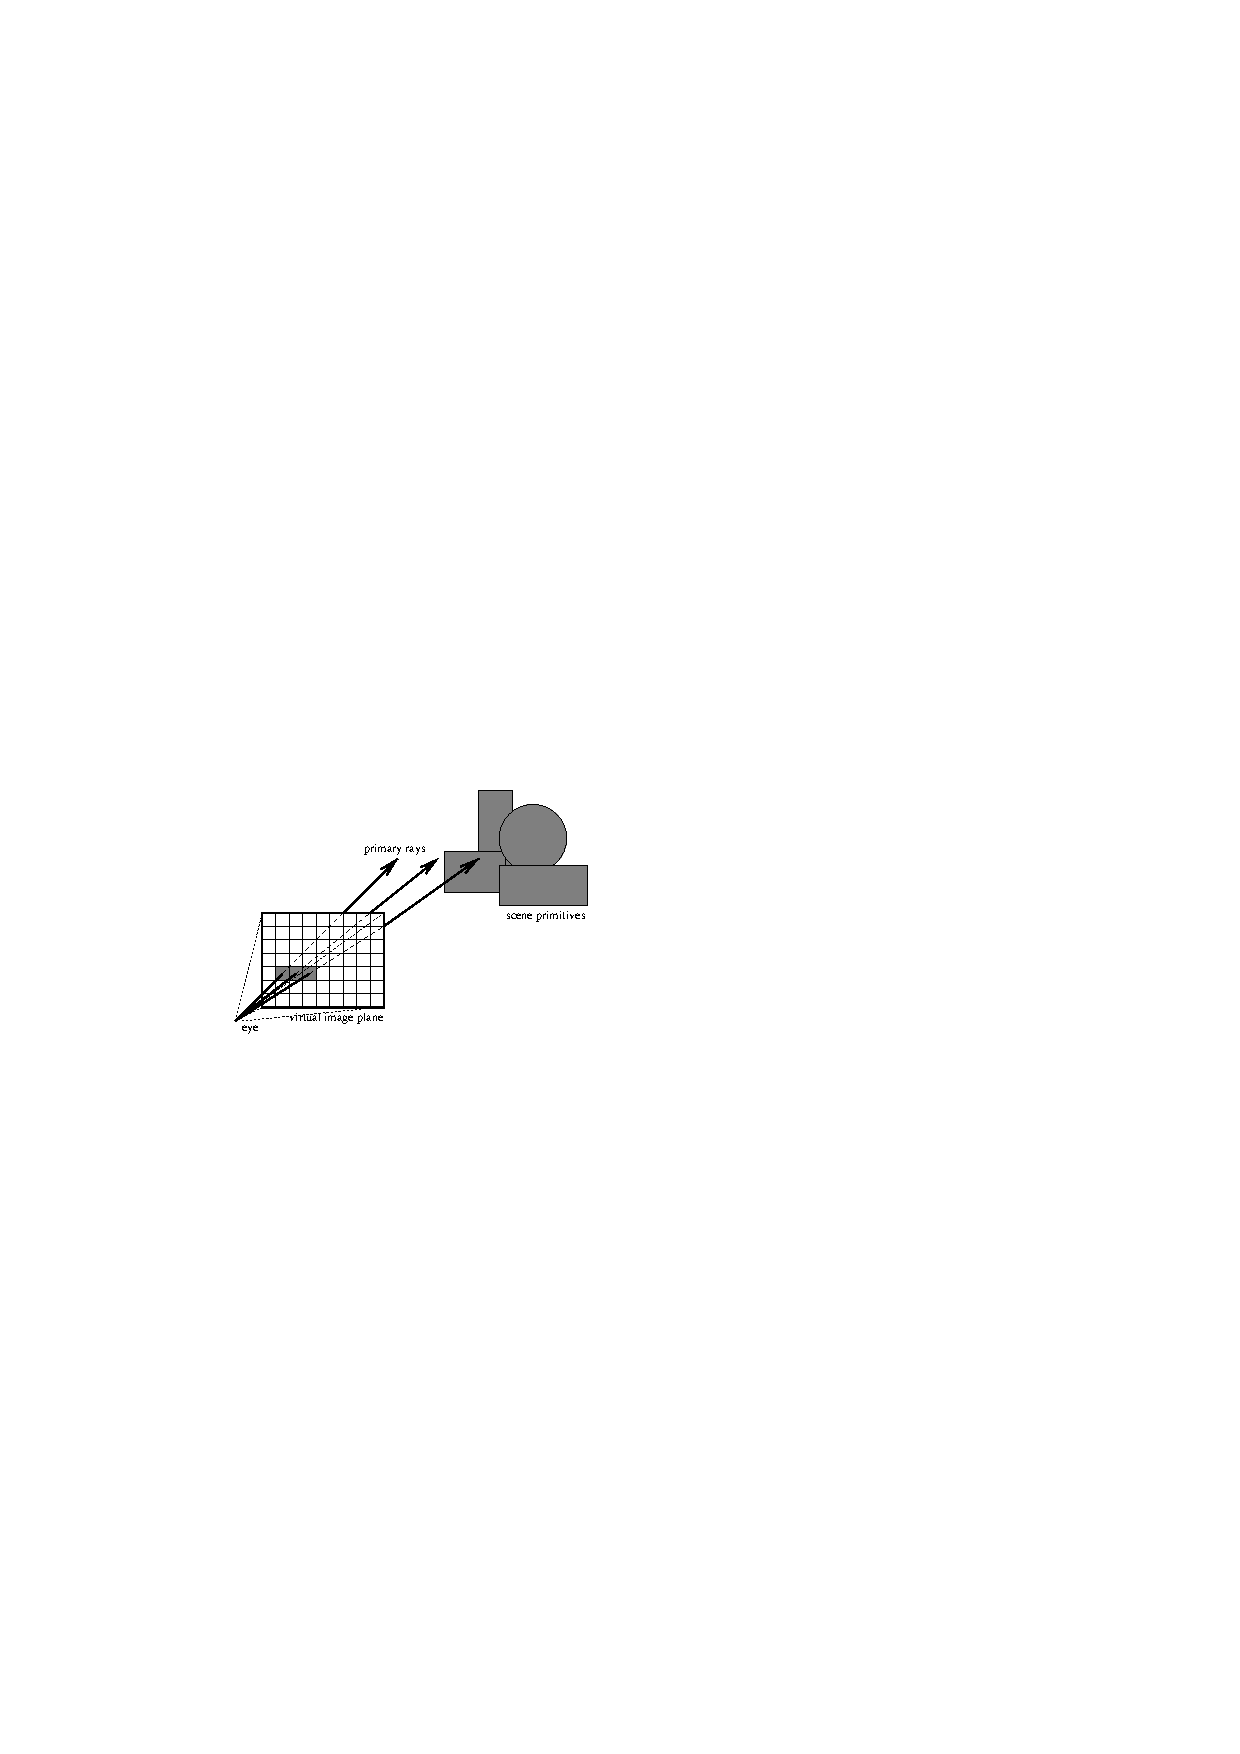
\includegraphics[width=0.42\linewidth]{figRayCastA.pdf}}}
			\hspace{0.01in} 
			\subfigure[]{
			\label{fig:RayCastingB}	%% label for second subfigure
			\fbox{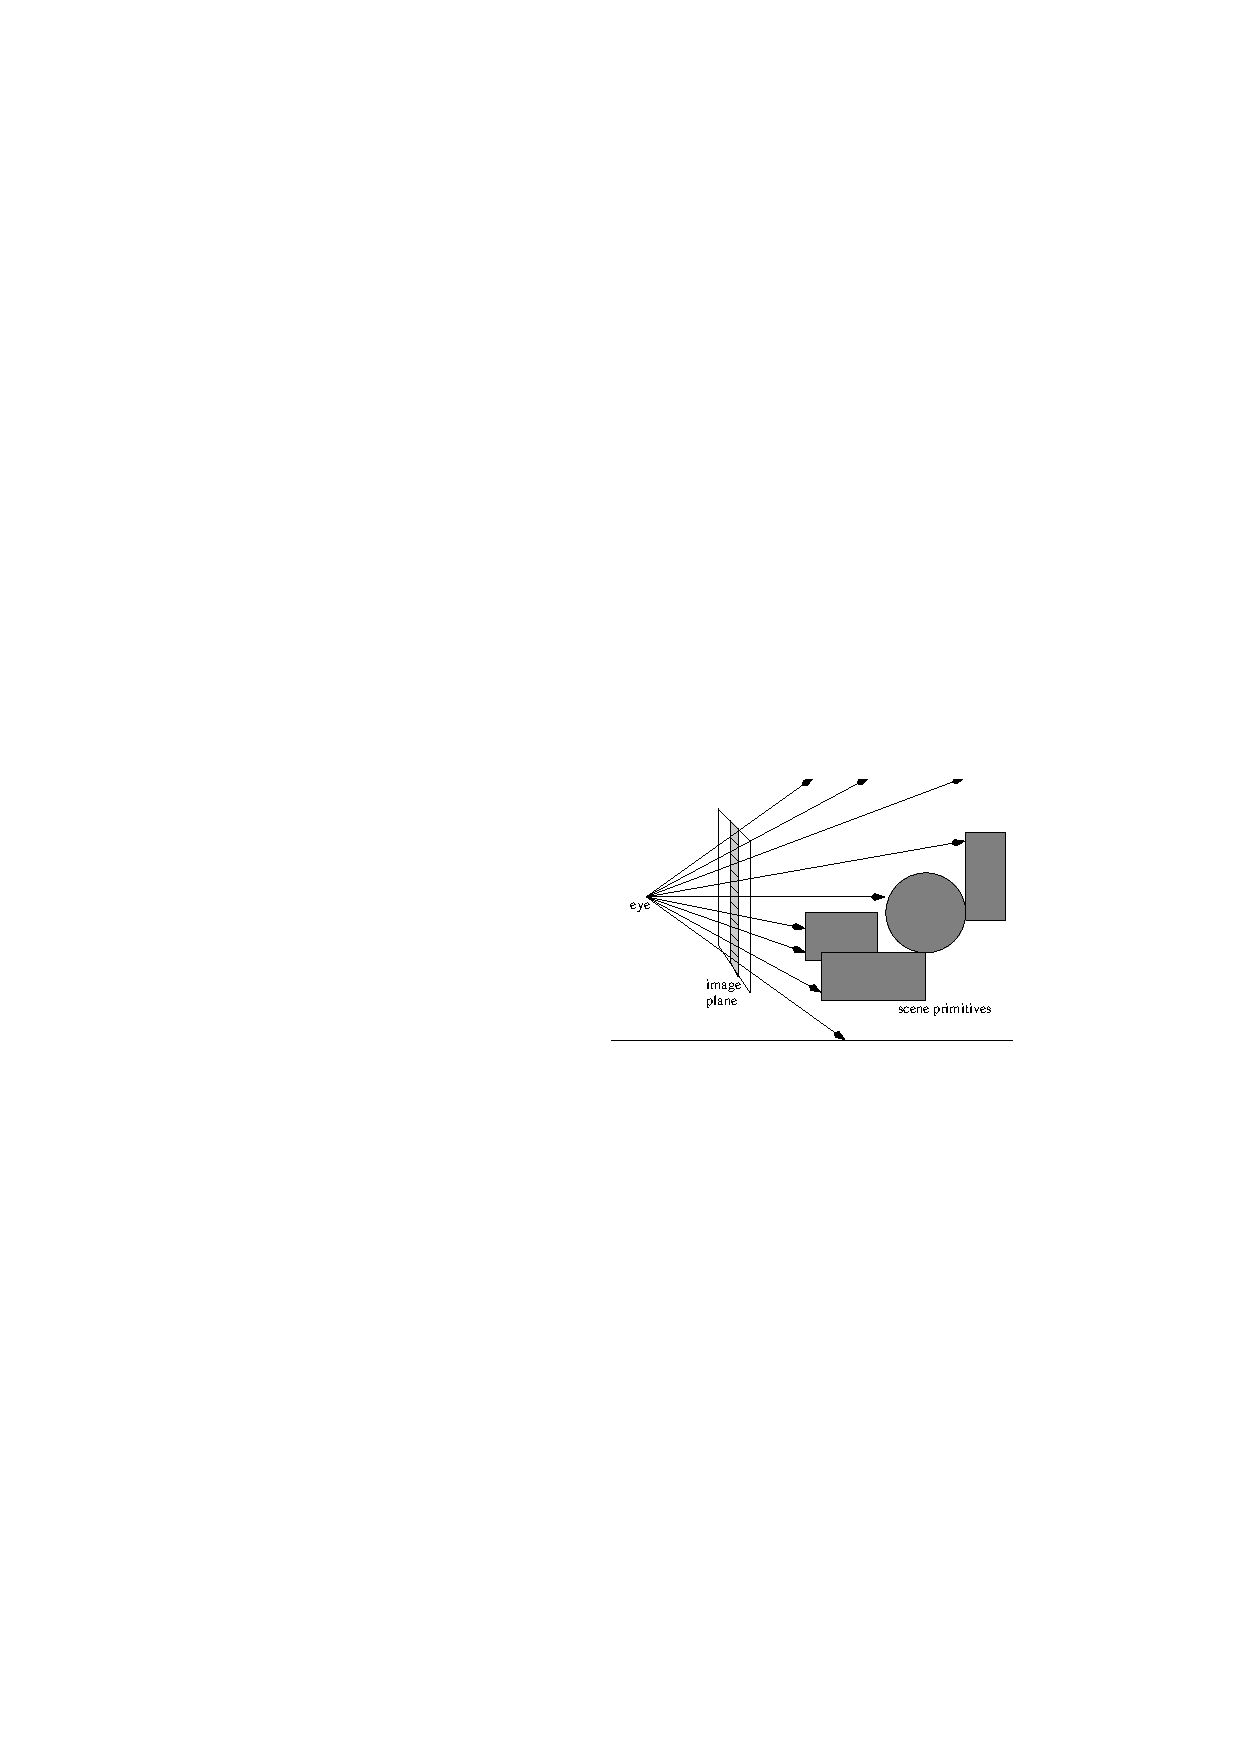
\includegraphics[width=0.45\linewidth]{figRayCastB.pdf}}}
			\renewcommand{\thefigure}{\thechapter.\arabic{figure}}
			\caption[Ray Casting]{\emph{The principle of ray casting: In order to compute an image of a scene, ``primary rays'' are shot from the camera, through each pixel of the virtual image plane, and cast into the scene (a). For each such ray, the closest object hit by this ray is determined by intersecting the ray with the geometric primitives that make up the scene (b).}} 
			\label{fig:ray_casting}	%% label for entire figure
		\end{figure}

	\item[Light and Visibility] \hfill \\

		In order to correctly support shadows, light sources only contribute to the incident illumination if the hit point is not occluded from the position of the respective light source, which is checked by tracing a shadow ray towards the direction of the light source.
		Additional to direct illumination from light sources, illumination from arbitrary other directions (e.g. from the reflection and refraction directions for specular effects) can be considered by casting a secondary ray into the respective direction and recursively evaluating the light being transported along this rays. This recursive evaluation then proceeds in exactly the same way as for the primary ray. Of course, these secondary rays can in turn trigger another recursion level of new rays, etc.


	\item[Ray-Surface Interaction] \hfill \\
		The appearance of a surface is determined by the how the surface interact with the light. The properties of the surface are typically abstracted as the \textit{material} which is actually a parameterized descriptions of the appearance at each point on the surface. These properties are modelled mathematically by the \textit{Bidirectional Reflectance Distribution Function} (BRDF). This function takes the incoming light direction, the outgoing light direction and the point hit by the light as the inputs, returns the amount of energy reflected by the surface at that point. 

	\item[Recursive Ray Tracing] \hfill \\
		The rays shot from the camera (termed as ''primary rays'') can be reflected about the surface normal at the intersection point and transmitted when intersect the transparent object, spawning secondary rays that ray-tracer need to recursively call the ray-tracing routine to trace, the contribution of the secondary rays will be added to the primary rays. 

		\begin{figure}[htp] 
			\centering 
			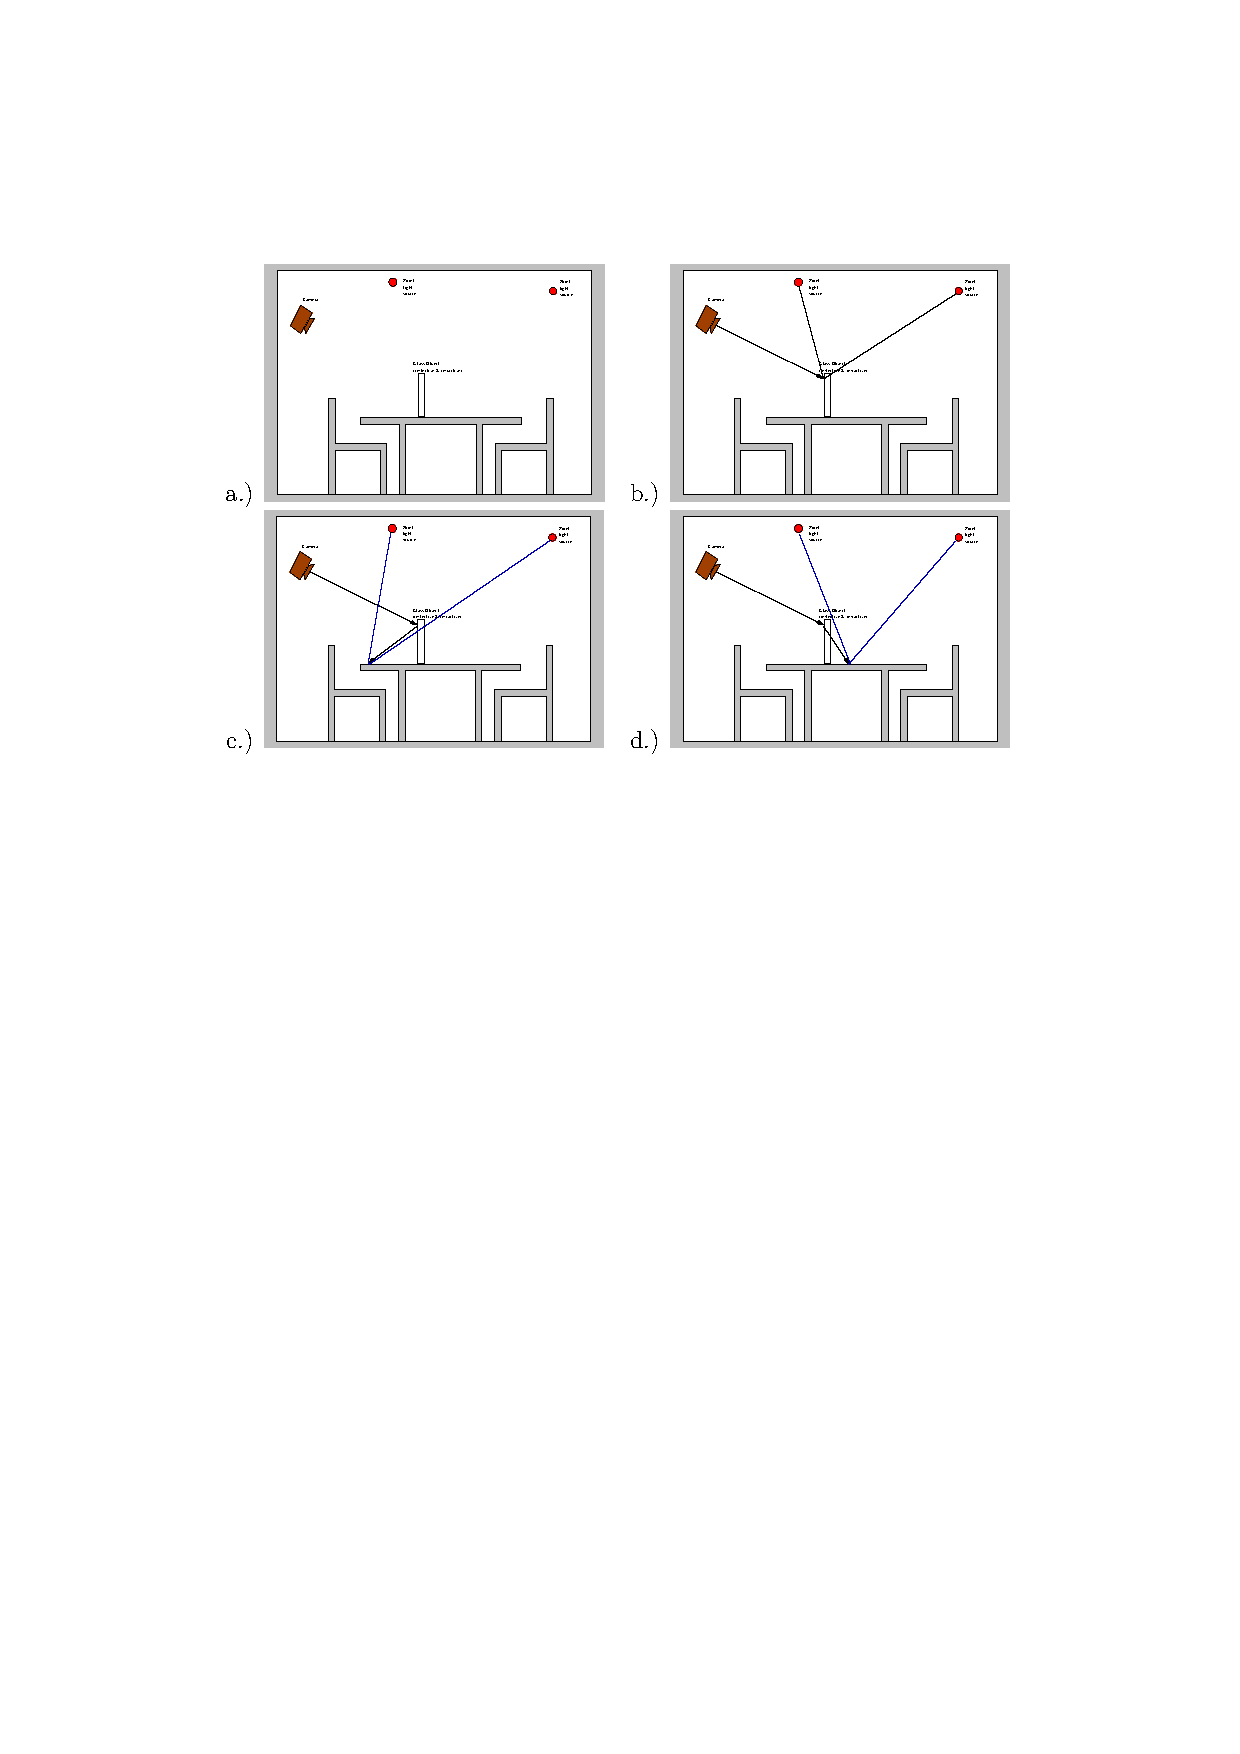
\includegraphics[scale=0.9]{figRayTracingRoom.pdf} 
			\renewcommand{\thefigure}{\thechapter.\arabic{figure}}
			\caption[Recursive Ray Tracing]{}
			\label{fig:ray_tracing_room} 
		\end{figure}

\end{description} 

\newpage

\section{Acceleration Structures}
The ray shooting algorithm which only uses a list of of all objects in the scene is also called a naive ray-shooting algorithm. It is a linear search process that tests the ray with all the objects and choose the one with the closest intersection found, if such an object exists. Thus the time complexity is \( O(n) \). As the scene complexity grows, the application using naive RSA runs unacceptably slowly. The straightforward approach to accelerate ray shooting algorithm is to reduce the number of unnecessary ray-primitive intersection tests. Thus we introduce the concept of acceleration structure.

The AS essentially is a kind of data structure which stores the spatial relationships of the geometric objects in the scene, thus it is also called \emph{spatial data structure}. The idea behind it is similar to accelerating other type of searching problem, if we can establish a kind of index structure which offers the relationship between the elements before performing query, lots of unnecessary tests can be skipped and the performance can be boosted. Over the last 20 years, many different kind of acceleration structures have been developed, however in principle these techniques mainly differ in whether they hierarchically organize the scene primitives (as done by Bounding Volume Hierarchy), or whether they subdivide the space into a set of non-overlapped voxels (as done by kd-trees or grids).  

Generally speaking, acceleration structures can be classified into two types by the approaches they adopt: spatial subdivision and object subdivision. Spatial subdivision approach subdivides the space into regions, hierarchically organizes the geometric objects which fall in the same spatial region into an object called \emph{cell}, and maintains the spatial relationships between the cells. When the ray shooting algorithm is performing, we test the ray against the cells instead of actual geometric objects, if the intersection is found, we go deep in this cell for further test, otherwise this cell will be skipped cause there is no chance that the ray can hit the any geometric objects in this cell, a significant number of intersection tests will be reduced. The most widely-used spatial subdivision structures are uniform grid and kd-tree. 

Object subdivision approach, on the other hand, logically breaks the object in the scene down into a set of objects groups, similar with building a scene graph. For example, a desk can be broke down into four legs and a surface, this forms a hierarchy structure to represent a desk object. If a ray does not hit the desk's bounding volume, there is no chance that the ray hits any parts of the desk and they will be culled, otherwise the ray will be recursively tested against each part of desk. The most widely-used structure of this approach is bounding volume hierarchy (BVH).

% Grid 
\subsection{Grid}

% What is Grid

% Grid Construction

% Grid Traversal

%Bounding Volume Hierarchy
\subsection{Bounding Volume Hierarchy}

% What is BVH 
Bounding volume hierarchy (BVH) are an acceleration structure based on primitive subdivision. The primitives are partitioned into a hierarchy of non-overlapped sets. In the hierarchy, the leaf node keeps the bounding volume of the attached primitive as the nodes' bounding volume, it also stores the actual primitive reference, while the interior node stores the bounding volume of its children node. When a ray is traversed through the tree, any time it misses a node's bounding volume, the entire sub-tree rooted by that node will be skipped. There are two important properties of BVH structure, one is that each primitive referenced by the hierarchy only once,  thus it will not be tested against the ray multiple times; the other one is that the memory consumption to represent the BVH is bounded. Figure ~\ref{fig:BVH} shows a simple scene and its corresponding BVH tree.

\begin{figure}[htp] 
	\fbox{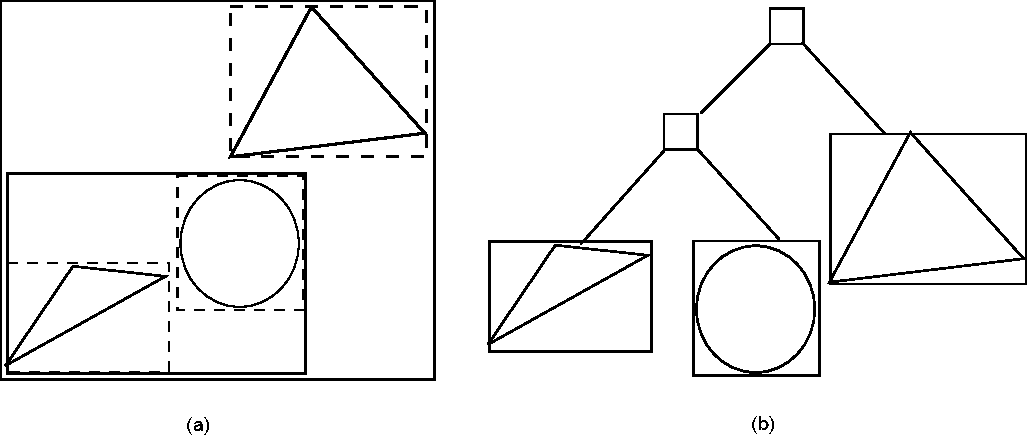
\includegraphics[scale=0.8]{figBVH.pdf}} 
	\renewcommand{\thefigure}{\thechapter.\arabic{figure}}
	\caption{Bounding Volume Hierarchy for a Scene}{(a) A simple scene containing several objects. The bounding boxes of the primitives are shown by dashed lines. The smaller triangle and the sphere are grouped together with a bounding box before being bounded by the bounding box that is corresponding the entire scene (both shown in solid box). (b) The corresponding bounding volume hierarchy, the root node stores the bounding box of the entire scene, it has two children node here, one is a leaf node with the bigger triangle attached, the other one is an interior node that encompasses the sphere and smaller triangle as leaf nodes. }
	\label{fig:BVH} 
\end{figure}

% BVH Construction 
\subsubsection{BVH Construction}
\label{subsubsec:bvh_construction}

Several stages are needed in the BVH construction process. 

\SetAlFnt{\small}
%\IncMargin{1em}
\begin{algorithm} 
	\SetKwInOut{Input}{input} \SetKwInOut{Output}{output}
	\Input{The collection of the primitives in the scene}
	\Output{The root node of BVH tree} 

	\Begin{
	\textit{Initialize the array for primitives}
	\textit{Recursively build BVH tree}
	\textit{Map the BVH tree to a compact linear representation}
	}
	\caption{Build BVH from primitives}
	\label{algo:BVH_construction} 

\end{algorithm}

Firstly, we and store centroid of the bounding box, the complete bounding box and the reference to the primitive for each primitive into an array as a working buffer.

Next, a partition procedure will be performed to split the primitive into two subsets and recursively build the BVH for the subsets. This produces a binary tree where each interior node holds the pointer to  its children nodes and each leaf node holds the references to one or a list of primitives. The partition step can be more complex, given \(n\) primitives, there are \( 2^n - 2 \) possible partitions, while many of them may lead to suboptimal BVH. Generally we choose the partition plane along a coordination axis, meaning that there are about \( 6n \) candidate partitions ( \( 2n \) partitions for each axis ). We use one axis of the three to place the partition. In practice, the axis with the greatest variation of bounding box centroid for the current set of primitives is a good choice. When choosing the position to place the partition plane, a general goal is to select a partition that doesn't have too much overlap of the bounding boxes of the two resulting primitive sets, this is based on the fact that overlapping of two primitive sets will cause the traversal of both children subtrees requiring more computation clipping collection of primitives. 

There are several schemes to choose where to place the partition: a simple method is to partition at the midpoint of the primitives' centroids along the splitting axis. However, this method may result a substantial overlap of two primitive subsets with certain distribution of primitives. Another straightforward but more adaptive partition scheme is to partition the primitives into two subsets with equal number of primitives. These two primitive partitioning approaches above can work well for some distributions of primitives, but they often choose the partitions leading to more nodes of the tree being traversed by the ray and hence unnecessarily ray-primitive intersection computations at rendering time. A more widely-used scheme used by best current algorithms for building acceleration structures are based on the ``surface area heuristic''  (SAH) model which provides a well-grounded cost model used to determine which of a number of partitions of primitives leading a better BVH for ray-primitive intersection tests. The SAH model will be discussed in depth in the chapter. As the partition has been fixed, we generate two interior nodes and classify the geometries into them by testing the primitives against the bounding volume the generated nodes.

Instead of only store the root node of the tree and visiting the nodes by manipulating the pointers, it is an important optimization to store the BVH tree into a compact linear array in depth-first array. This representation makes the BVH traversal more cache-friendly thus improves the overall performance. In the memory, the first child of each interior node is right next to the interior node, for the second child node, the offset to it is stored explicitly in the data structure of BVH tree node. See Figure ~\ref{fig:bvh_linear_layout} for an illustration of the topology of BVH tree nodes and its representation in memory.   

\begin{figure}[htp] 
	\centering 
	\fbox{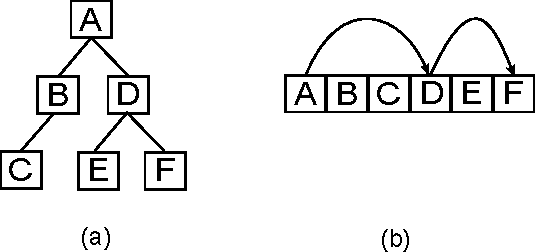
\includegraphics[scale=0.8]{figBVHLinearLayout.pdf}}
	\renewcommand{\thefigure}{\thechapter.\arabic{figure}}
	\caption[Linear Layout of a BVH in memory]{(a) The topology of the nodes in BVH tree. (b) The memory layout of the nodes of the BVH tree. The nodes are stored in depth-first order.}
	\label{fig:bvh_linear_layout}
\end{figure}

% BVH Traversal
\subsubsection{BVH Traversal}
\label{subsubsec:bvh_traversal}
The traversal of BVH is a simple process, the ray is tested against the bounding volume of the node in the tree from the root node which represents the entire scene down to the leaf nodes.  If an intersection occurs (including the case that the ray starts inside of the node), for an interior node, a down traversal is performed to visit the children nodes and save the far node onto a stack, for a leaf node, each primitive will be tested against the ray. If there is no intersection, no further test will be be performed in the current sub-tree and the next node to be visited is retrieved from the stack (or finish the traversal if the stack is empty). The intersection test between the ray and bounding volume is fast, take bounding box for example, ray-box is fast ray-slab test \cite{kk1986}. 

\SetAlFnt{\small}
%\IncMargin{1em}
\begin{algorithm} 
	\SetKwData{RootNode}{root} \SetKwData{Node}{node} \SetKwData{Stack}{stack}
	\SetKwData{NodeIndex}{nodeIndex} 
	\Begin{
		\tcp{Initialise the stack, push the root node} 
		push $root$ onto $stack$  
		\While{true} {
			\tcp{Retrieve the top node of the stack}	
			$node \longleftarrow stack[nodeIndex]$ \\	
			\If{the ray intersects the bounding box of the current node} {
				\If{$node$ is leaf node} { 
					\textit{Intersect ray with primitives in leaf node} 	
				}
				\Else{
					\textit{Put far BVH node on $stack$, advance to near node}
				}
			}
			\Else{
				\If{$stack$ is empty} {break}
				\textit{Advance $nodeIndex$}
			}
		}
	}
	\caption{BVH Traversal}
	\label{algo:bvh_traversal} 
\end{algorithm}


% KD-Tree
\subsection{KD-Tree}
Before introducing kd-tree, a short introduction to \textit{Binary Space Partitioning} (BSP) tree has to be made. A BSP tree is a data structure developed in the purpose of solving the hidden surface removal problems in computer graphics. The binary space partitioning is a process of adaptively and recursively subdivide the voxel of the scene into irregular sized regions with a chosen split plane until a termination criteria has been satisfied. Different scheme of choosing the split plane leads to two major variants of BSP tree, polygon-aligned form and axis-aligned form. The polygon-aligned form chooses the plane aligning the polygon in the scene as the split plane, while axis-aligned form always chooses the planes perpendicular to a certain coordinate axis. The kd-tree is actually the axis-aligned form of the BSP tree which makes both traversal and construction of the tree more efficient. We will focus on kd-tree here in this thesis.

\begin{figure}[H] 
	\centering
	\fbox{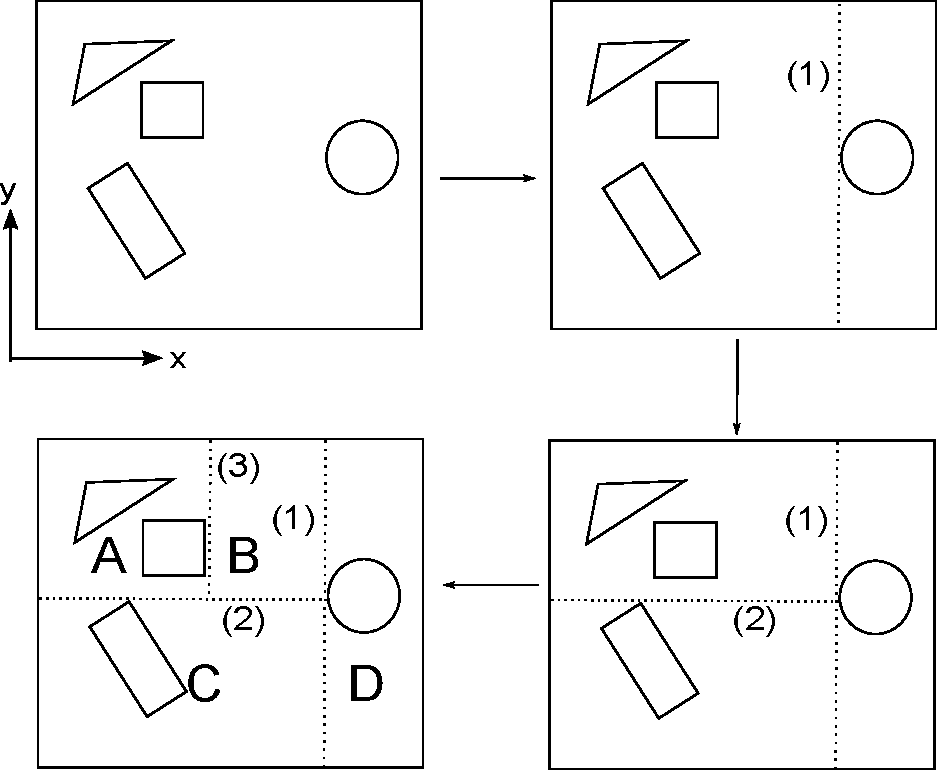
\includegraphics[scale=0.8]{figKDTreeSubdivide.pdf}} 
	\renewcommand{\thefigure}{\thechapter.\arabic{figure}}
	\caption[2D view of the subdivision of a scene]{The top view of a scene which is recursively subdivided by the split planes (shown in dashed lines and labeled by numbers) into several small regions (labeled by the letters).}
	\label{fig:kd-tree_subdivide} 
\end{figure}

Figure ~\ref{fig:kd-tree_subdivide} provides an overview of how the scene is recursively subdivided along one of the coordinate axes. In the figure, a scene is recursively subdivided by 3 split planes. Initially, the entire scene as the root node of the tree, the first split is along the \(x\) axis and it subdivides the scene into two regions. Then the left region is refined a few more times with the number 2 splitting plane. In the subdivision process, some criteria such as which axis is used to place the splitting planes,  at which position along the axis the plane is placed and at what point subdivision terminates can all substantially affect the performance of the kd-tree in practice.  

%then termination test is performed to see if the partitioning should be stopped, in this case we continue subdivision, thus the newly generated voxels left and right become the children of the root node. Next step we split the left node into two voxels and assume the termination criteria has been satisfied, the subdividing should be stopped here, thus the new child nodes becomes the leaf node of the kd-tree, as labeled by ``A'' and ``E''. Any Internal node has the references to its child nodes and the leaf nodes will contain a list of primitives which fall in the spatial region covered by the leaf node. The primitive which straddles a split plane will belong to all the nodes it intersects with.

\begin{figure}[H]
	\centering
	\fbox{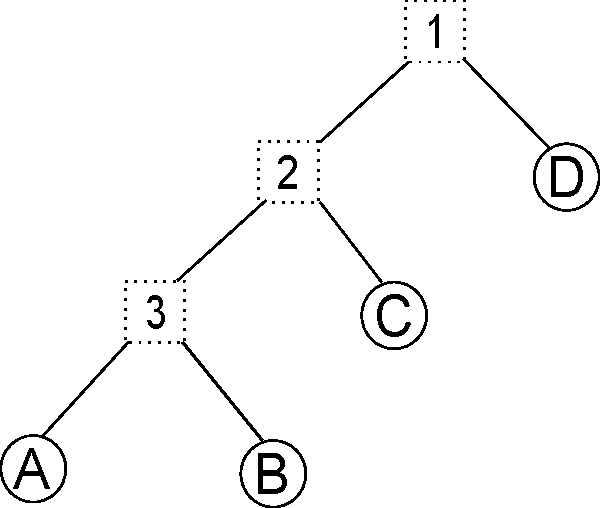
\includegraphics{figKDTreeSubdivideTree.pdf}} 
	\renewcommand{\thefigure}{\thechapter.\arabic{figure}}
	\caption[KD-Tree representation of a simple scene]{The kd-tree built from the scene in Figure \ref{fig:kd-tree_subdivide}}
	\label{fig:kd-tree_subdivide_tree} 
\end{figure}

% Why kd-tree
%KD-Trees are useful data structure for the searching problems which RSA requires, nearest neighbor search (NNS). Because it essentially sorts the primitives into two sets, the one in front of the split plane and those behind, relative to the origin of a given ray, we can determine the which set of primitives is nearer to the origin, and which is further. To find the closest primitive hit by the ray, we simply perform a down-traversal in a front-to-back order on the kd-tree built from the scene, when the leaf node is reached, a linear search will be required to find the primitive with the minimum distance to the origin of the ray. Furthermore, since the split planes are orthogonal to the coordinate axis, the intersection test between the ray and splitting plane has been greatly simplified. 

% KD-Tree Representation
\subsubsection{KD-Tree Data Representation}
As a special case of binary tree, the node of kd-tree has the similar representation. Each interior node has to contain the following three data fields: 
\begin{itemize}\itemsep1pt
	\item{Split axis: which axis is used to to place the splitting plane for this node}
	\item{Split position: the position of the splitting plane along the splitting axis}
	\item{Reference to children nodes: information associates to the children of this nodes}
\end{itemize}
While each leaf nodes only contains the reference to the collection of primitives attached to it. Both leaf nodes and interior nodes share a common data filed which is a flag indicating the this node is a leaf or interior. 

In practice all these data fields can be put in a compact data structure which consume 8 bytes (assuming the system uses 4-byte floating point values and pointers) regardless if the node is an interior or a leaf node using the \textbf{union} in C/C++ programming language. They share the same memory location using one bit of data to indicate it is leaf node or interior and the node-specific data is encoded into a 4-byte unsigned integer value. For interior node, 

\begin{lstlisting}[caption=Data layout of kd-tree node, label=lst:kd-tree_node]
	struct KDTreeLeaf{
		unsigned int flag; 
		// bits 0..30  	: offset bits
		// bit 31(sign) : flag whether node is a leaf  
	}
	struct KDTreeInterior{
		float split; 
		unsigned int flag; 
		// bits 0..1 	: splitting dimension
		// bits 2..30 	: offset bits
		// bit 31(sign) : flag whether node is a leaf
	}
	union KDTreeNode{ 		
		struct KDTreeLeaf;
		struct KDTreeInterior; 
	}
\end{lstlisting}

% kd-tree construction
\subsubsection{KD-Tree Construction}
\label{subsubsec:kd-tree_construction}
A kd-tree construction essentially is a process of recursively subdivide the current spatial region into two subregions with a certain axis-aligned split plane that is selected using a particular strategy. The construction process starts with the extend of the entire scene. Initially, the root node is leaf node, and all newly generated nodes are also leaf nodes, when a node is split by split plane, it will become an interior node, and the objects associated with it will be sorted to into its two new descendants. 

The recursion will be terminated when a certain termination criteria is reached. Commonly we use the maximum depth of the recursion or a pre-defined threshold of the number of the primitives attached to a leaf node as the termination criteria. In practice, the value \(8 + 1.3\log(N)\) is found a reasonable maximum depth of the tree for a variety of scenes \cite{ph2004}.The construction of kd-tree is described in pseudo-code in Algorithm \ref{algo:kd-tree_construction}.


% Begin the algorithm: kd-tree construction
\SetAlFnt{\small}
\begin{algorithm}[H]

	\SetKwData{triangleList}{\(T\)}
	\SetKwData{triangleListLeft}{\(T_{L}\)}	
	\SetKwData{triangleListRight}{\(T_{R}\)}

	\SetKwData{voxel}{\(V\)}
	\SetKwData{voxelLeft}{\(V_{L}\)}
	\SetKwData{voxelRight}{\(V_{R}\)}
	\SetKwData{currentNode}{\(node\)}
	\SetKwData{currentBox}{\(box\)} 
	\SetKwData{splitPlane}{\(p\)}

	\SetKwFunction{CalcBounds}{\ProcNameSty{CalcBounds}}
	\SetKwFunction{FindSplitPlane}{\ProcNameSty{FindSplitPlane}}
	\SetKwFunction{ClassifyTriangles}{\ProcNameSty{ClassifyTriangles}}
	\SetKwFunction{SAHCost}{\ProcNameSty{SAHCost}}
	\SetKwFunction{KDTreeBuildRec}{\ProcNameSty{KDTreeBuildRec}}
	\SetKwFunction{BuildRec}{\ProcNameSty{BuildRec}}
	\SetKwFunction{Terminate}{\ProcNameSty{Terminate}}
	\SetKwFunction{CreateLeafNode}{\ProcNameSty{CreateLeafNode}}
	\SetKwFunction{CreateNode}{\ProcNameSty{CreateNode}}
	
	\myfunc \BuildRec{\triangleList, \voxel} \newline 
	\Begin {
		\If {\Terminate{\triangleList, \voxel}}	{
			\Return \CreateLeafNode{\triangleList}\; 
		}
		
		\splitPlane = \FindSplitPlane{\triangleList, \voxel}\;
		(\voxelLeft, \voxelRight) = Split \voxel with \splitPlane\;
		(\triangleListLeft, \triangleListRight) = \ClassifyTriangles{\triangleList, \voxelLeft, \voxelRight, \splitPlane}\;
		
		\Return \CreateNode{\splitPlane, \BuildRec{\triangleListLeft, \voxelLeft}, \BuildRec{\triangleListRight, \voxelRight}}\;
	}

	\myalgblankline
	
	\myfunc \KDTreeBuildRec{\triangleList} \newline
	\Begin {
		\voxel = \CalcBounds{\triangleList}\;
		\Return \BuildRec{\triangleList, \voxel}\;
	}

	\caption{Recursive KD-tree construction}
	\label{algo:kd-tree_construction}
\end{algorithm}


As shown in the above algorithm, in each partition of the current node, a split plane has to be selected, this is done by the function \emph{FindSplitPlane}. For a kd-tree, a split plane can be positioned arbitrarily, as long as they are perpendicular to one of the \( {x, y, z} \) axis. However, different strategy of choosing the split plane may lead to a considerable performance gap up to a factor of two of more when traversing the built kd-tree \cite{havran200}. More detail will be discussed in chapter 3. 

\subsubsection{KD-Tree Traversal}
\label{subsubsec:kd-tree_traversal}
%kd-tree traversal
% 1. Motivation
% 2. Describe with figures
% 3. Pseudocode 

Given a ray \(R\) and a kd-tree, the kd-tree traversal is a procedure that identify the sequence of the kd-tree leaves intersected by the ray. There are several types of traversal algorithms developed, such as sequential, recursive and those with neighbor-links. Due to the simplicity, here we only describe the recursive traversal algorithm. The traversal is in a top-down fashion, starting from the root node, recursively descends the branches of the kd-tree along the ray path. Before going into any details of the ray traversal algorithm, a few terminologies have to be introduced, For each interior node the ray visits, the mutual position of the origin of a ray and the axis-aligned box \( AB(s) \) of this node has to be considered. The first configuration is when the origin of a ray is located outside, also known as ``the ray with external origin'', and the other one is when the origin of the ray is inside the \( AB(s) \), we call it ``the ray with internal origin''. When a bounding box is intersected by a ray \( R \), there are two important points along the ray path which can be expressed by two signed distance. The point where \( R \) enters the bounding box is called \emph{entry point}, corresponding to the \emph{entry signed distance}. The point where R leaves the bounding box is called \emph{exit point}, corresponding to the \emph{exit signed distance}. 

When the ray enters a kd-tree node (one traversal step), the intersection between the ray and the bounding box associating to the current node creates a parameter interval \( t_{near}, t_{far} \) which are the signed distance of the entry and exit point. Intersecting the ray with bounds of the entire scene (the tree's root node) gives the initial \( t_{near}, t_{far} \), then the parameter interval is updated incrementally during the traversal. If the ray misses the overall bounding box ( \( t_{near} > t_{far} \) ), then the traversal can exit immediately. 

If the current node is a leaf node, each primitive attached is tested against the ray and update a parameter \( t_{closest} \) to find the closest intersection point. 

If the current node is an interior node, it has to determine which of the two children the ray enters first. We calculate the parametric distance \(d\) to the splitting plane of the node in the same manner as was done in computing the intersection of a ray and axis-aligned plane for the ray-bounding box test, \( d = (t_{split} - r_{origin}[dim]) / r_{dir}[dim] \), and then compare \(d\) to the current ray segment \( t_{near}, t_{far} \). If the ray segment lies completely on one side of the splitting plane ( \( d >= t_{far}\ or\ d <= t_{near}\) ), the subtree on the other side can be skipped immediately and the traversal will continue to proceed to the corresponding child voxel. Figure \ref{fig:kd-tree_traversal_one_child} shows some configurations of this case. 

\begin{figure}[hpt]
	\centering
	\fbox{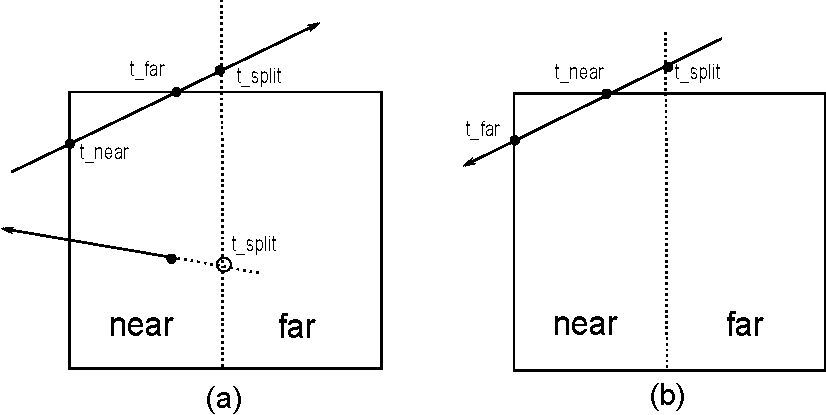
\includegraphics{figKDTreeTraversalOneChild.pdf}}
	\renewcommand{\thefigure}{\thechapter.\arabic{figure}}
	\caption[KD-tree traversal proceed only one child node] {Two cases where the traversal will only proceed one child node. }
	\label{fig:kd-tree_traversal_one_child}	%% label for entire figure
\end{figure}
 
If none of the children nodes can be culled, the position of the ray's origin with respect to the splitting plane is enough to determine which of the child node is closer in turn should be visited first, figure \ref{fig:kd-tree_traversal_children} illustrate this case.  

\begin{figure}[H]
	\centering
	\fbox{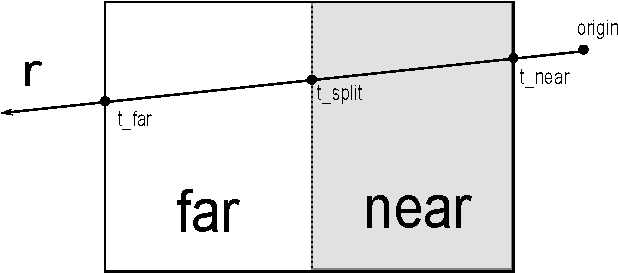
\includegraphics{figKDTreeTraversalChildren.pdf}}
	\renewcommand{\thefigure}{\thechapter.\arabic{figure}}
	\caption[KD-tree traversal proceed both children nodes] {The children nodes are labeled as ``near'' and ``far'' by checking \( t_{split} - r_{origin}[dim] \). If it is positive, the ray enters the left node first; otherwise the right node is the ``near'' node.  The parameter interval for traversal the ``near'' and ``far'' node are \( t_{near}, t_{split} \), \( t_{split}, t_{far} \) repectfully. }
	\label{fig:kd-tree_traversal_children}	%% label for entire figure
\end{figure}

Figure \ref{fig:kd-tree_traversal} shows the basic process of ray traversal through the tree. 
\begin{figure}[hpt]
	\centering
	\fbox{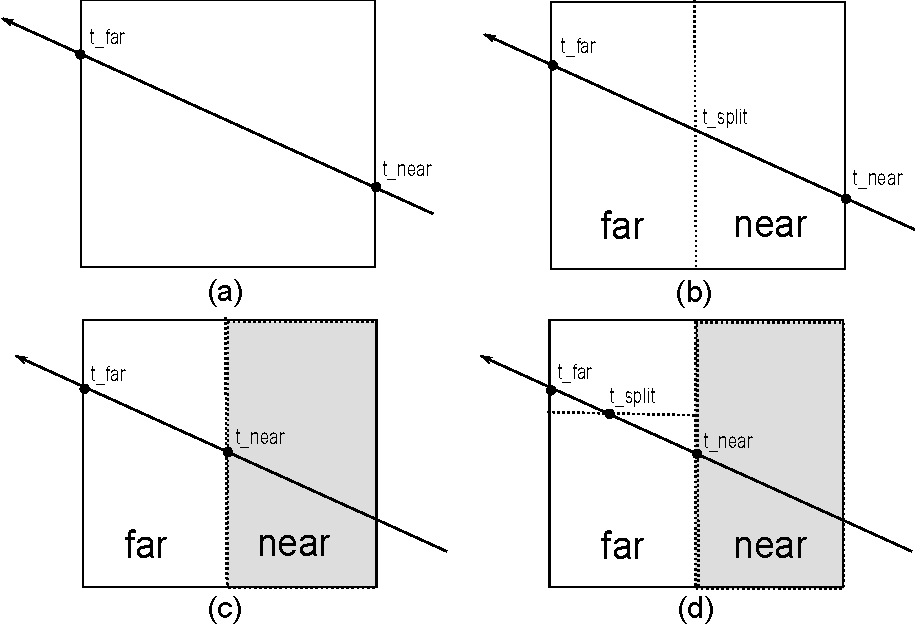
\includegraphics[width=\linewidth]{figKDTreeTraversal.pdf}}
	\renewcommand{\thefigure}{\thechapter.\arabic{figure}}
	\caption[Traversal of Ray Through the KD-Tree.]{(a) The ray intersects against the bounding box of the kd-tree. The two intersection points can be simply represented by a parametric range \([t_{near}, t_{far}]\). (b) Assume this node is an interior node, it is necessary to consider the two children nodes. The node that the ray enters first is labeled as ``near'', corresponding the range \([t_{near}, t{split}]\). If the near node is leaf node which contains geometric primitives, ray-primitives intersection tests will be performed; otherwise, its children nodes will be processed. (c) If no intersection found in the near node, then the far node (on the left) is processed. (d) The traversal process will continue in a depth-first, front-to-back order, until the closest intersection is found or the ray exits the tree.	
	} % end of caption
	\label{fig:kd-tree_traversal}	%% label for entire figure
\end{figure}

% The algorithm 
\SetAlFnt{\small}
\begin{algorithm}[H]
	% Variables 
	\SetKwData{ray}{\(r\)}
	\SetKwData{rayOrigin}{\(r.origin\)}
	\SetKwData{rayOriginDim}{\(r.origin[node.dim]\)}
	\SetKwData{rayDirection}{\(r.dir\)}
	\SetKwData{rayDirectionDim}{\(r.dir[node.dim]\)}
	\SetKwData{tNear}{\(t_{near}\)}
	\SetKwData{tFar}{\(t_{far}\)}
	\SetKwData{tClosest}{\(t_{closest}\)}
	\SetKwData{tHit}{\(t_{hit}\)}
	\SetKwData{D}{\(d\)}	

	\SetKwData{rootNode}{\(rootNode\)}
	\SetKwData{node}{\(node\)}
	\SetKwData{nodeSplit}{\(node.split\)}
	
	% Functions
	\SetKwFunction{KDTreeTraversalRecFunc}{\ProcNameSty{KDTreeTraversalRec}}
	\SetKwFunction{TraversalRecFunc}{\ProcNameSty{TraversalRec}}
	\SetKwFunction{RayBoxIntersectionFunc}{\ProcNameSty{RayBoxIntersection}}
	\SetKwFunction{RetrieveFarNodeFunc}{\ProcNameSty{RetrieveFarNode}}
	\SetKwFunction{RetrieveNearNodeFunc}{\ProcNameSty{RetrieveNearNode}}
	
	\myfunc \KDTreeTraversalRecFunc{\ray, \rootNode} \newline
	\Begin{
		{\tNear, \tFar} $\leftarrow$ \RayBoxIntersectionFunc{\ray, \rootNode}\;
		\If {\tNear > \tFar} {
			\tcp{The ray misses the bounding box}
			\Return\; 
		}
		
		\TraversalRecFunc{\rootNode, \tNear, \tFar}\; 
	}
	
	\BlankLine \BlankLine 

	\myfunc \TraversalRecFunc{\node, \tNear, \tFar} \newline
	\Begin{
		Initiailise \tClosest to the maximum distance\; 
		\If { \node is leaf node} { 
			Intersect all the primitives in the node against the ray\; 
			\Return \tClosest\;
		}
		\D $\leftarrow$ (\nodeSplit - \rayOriginDim) / \rayDirectionDim \;
		\If {\D <= \tNear} {
			\tcp{Cull the ``near'' node}
			\Return \TraversalRecFunc{ \RetrieveFarNodeFunc{\node}, \tNear, \tFar}\; 
		}
		\ElseIf {\d >= \tFar} {
			\tcp{Cull the ``far node}
			\Return \TraversalRecFunc{ \RetrieveNearNodeFunc{\node}, \tNear, \tFar}\;
		}
		\Else {
			\tcp{Need to proceed both children nodes}
			\tHit $\leftarrow$ \TraversalRecFunc{\RetrieveNearNodeFunc{\node}, \tNear, \D}\;
			\If {\tHit <= \D} {
				\Return \tHit\; 
			}
			\Return \TraversalRecFunc{\RetrieveFarNodeFunc{\node}, \D, \tFar}\;
		}
	}
	\caption{Recursive KD-Tree Traversal}
	\label{algo:kdtree_traversal_rec}
\end{algorithm}





